\documentclass{llncs}
\usepackage{hyperref}
\usepackage{url}
\pagestyle{plain}
\usepackage{threeparttable}
\input{math_commands.tex}
%\usepackage[latin9]{inputenc}
%\usepackage[T1]{fontenc}
\usepackage{float}
\usepackage{wrapfig}
\usepackage{lineno}
\usepackage{amsmath}
\usepackage{amssymb}
\usepackage{graphicx}
\usepackage{subcaption}
\usepackage{tabularx}
\usepackage{cases}
\captionsetup{compatibility=false}
% \usepackage{esint}
\usepackage{array}
\usepackage{epstopdf}
\usepackage{placeins}
\usepackage{pgfplots}
\usepackage{url}
\usepackage{tikz}
\usepackage{calc}
\usepackage{array}
\usepackage[linesnumbered,ruled,vlined]{algorithm2e}
\usetikzlibrary{positioning, arrows.meta,calc}

%%%%%%%%%%%%%%%%%%%%%%%%%%%%%%%
%%%%%%%%%%%%%%%%%%%%%%%%%%%%%%%

\newcommand{\vW}{\boldsymbol{W}}
\newcommand{\val}{{\textrm{value}}}
\newcommand{\Val}{{\textrm{value}}}
\newcommand{\MILP}{{\textrm{MILP}}}
\newcommand{\LP}{{\textrm{LP}}}
\newcommand{\Improve}{\mathrm{Improve}}
\newcommand{\Utility}{\mathrm{SAS}}
\newcommand{\Sol}{\mathrm{Sol}}
\newcommand{\sol}{\mathrm{sol}}
\newcommand{\UB}{\mathrm{UB}}
\newcommand{\LB}{\mathrm{LB}}
\newcommand{\ub}{\mathrm{ub}}
\newcommand{\lb}{\mathrm{lb}}
\newcommand{\B}{\mathrm{B}}
\usepackage{amsmath, amssymb, amsfonts}
\newcommand{\ReLU}{\mathrm{ReLU}}
\newcommand{\CMP}{{\textrm{CMP}}\ }
\newcommand{\fix}{\marginpar{FIX}}
\newcommand{\new}{\marginpar{NEW}}
\newcommand{\toolname}{Hybrid MILP}


\title{Global case}
\date{}


\begin{document}
	
	\maketitle
	\linenumbers
	\begin{abstract}
		TODO
	\end{abstract}
	
	\section{Introduction}
	
	\section{Notations and Preliminaries}
	
	In this paper, we will use lower case latin $a$ for scalars, bold $\boldsymbol{z}$ for vectors, 
	capitalized bold $\boldsymbol{W}$ for matrices, similar to notations in \cite{crown}.
	To simplify the notations, we restrict the presentation to feed-forward, 
	fully connected ReLU Deep Neural Networks (DNN for short), where the activation function is $\ReLU : \mathbb{R} \rightarrow \mathbb{R}$ with
	$\ReLU(x)=x$ for $x \geq 0$ and $\ReLU(x)=0$ for $x \leq 0$, which we extend componentwise on vectors.
	
	%In this paper, we will not use tensors with a dimension higher than matrices: those will be flattened.
	
	%\subsection{Neural Network and Verification}
	
	
	% testtesttesttest
	An $\ell$-layer DNN is provided by $\ell$ weight matrices 
	$\boldsymbol{W}^i \in \mathbb{R}^{d_i\times d_{i-1}}$
	and $\ell$ bias vectors $\vb^i \in \mathbb{R}^{d_i}$, for $i=1, \ldots, \ell$.
	We call $d_i$ the number of neurons of hidden layer $i \in \{1, \ldots, \ell-1\}$,
	$d_0$ the input dimension, and $d_\ell$ the output dimension.
	
	Given an input vector $\boldsymbol{z}^0 \in \mathbb{R}^{d_0}$, 
	denoting $\hat{\boldsymbol{z}}^{0}={\boldsymbol{z}}^0$, we define inductively the value vectors $\boldsymbol{z}^i,\hat{\vz}^i$ at layer $1 \leq i \leq \ell$ with
	\begin{align*}
		\boldsymbol{z}^{i} = \boldsymbol{W}^i\cdot \hat{\boldsymbol{z}}^{i-1}+ \vb^i \qquad \, \qquad
		\hat{\boldsymbol{z}}^{i} = \ReLU({\boldsymbol{z}}^i).
	\end{align*} 
	
	The vector $\hat{\boldsymbol{z}}$ is called post-activation values, 
	$\boldsymbol{z}$ is called pre-activation values, 
	and $\boldsymbol{z}^{i}_j$ is used to call the $j$-th neuron in the $i$-th layer. 
	For $\boldsymbol{x}=\vz^0$ the (vector of) input, we denote by $f(\boldsymbol{x})=\vz^\ell$ the output. Finally, pre- and post-activation neurons are called \emph{nodes}, and when we refer to a specific node/neuron, we use $a,b,c,d,n$ to denote them, and $W_{a,b} \in \mathbb{R}$ to denote the weight from neuron $a$ to $b$. Similarly, for input $\boldsymbol{x}$, we denote by $\val_{\boldsymbol{x}}(a)$ the value of neuron $a$ when the input is $\boldsymbol{x}$.	For convenience, we write $n < z$ if neuron $n$ is on a layer before $\ell_z$, and $n \leq z$ if $n< z$ or $n=z$.
	
	Concerning the verification problem, we focus on the global-robustness question. Global robustness asks to determine how the output of a neural network will be affected under a certain kind of small perturbations to any possible input. In this view, Lipschitz continuity is a good characterization of global robustness.
	
	
	Recall the definition of Lipschitz continuity:
	 under distance $d$, a function $f(x)$ is Lipschitz continuous with respect to constant $K$ if:
	\begin{align*}
		\forall \boldsymbol{x} \forall\boldsymbol{y} (|f(\boldsymbol{x}) -f(\boldsymbol{y}) |\leq K|\boldsymbol{x}-\boldsymbol{y}|)
	\end{align*} 
	In our practice of global robustness, we will consider the following weaker property with respect to a certain number $\epsilon$:
	\begin{align*}
		\forall \boldsymbol{x} \forall\boldsymbol{y} &  (|\boldsymbol{x}-\boldsymbol{y}| \geq \epsilon \implies|f(\boldsymbol{x}) -f(\boldsymbol{y}) |\leq K|\boldsymbol{x}-\boldsymbol{y}|\\
		&  |\boldsymbol{x}-\boldsymbol{y}| < \epsilon \implies|f(\boldsymbol{x}) -f(\boldsymbol{y}) |\leq K\epsilon)
	\end{align*} 
	In terms of the code, it is compute an optimization question respect to a certain number $\epsilon$:	\begin{align}\label{global_robustness}
			\max_{|\boldsymbol{x}-\boldsymbol{y}| \leq \epsilon} |f(\boldsymbol{x}) -f(\boldsymbol{y}) |
	\end{align} We can use this maximum value to estimate the Lipschitz constant.
	
	\section{Local robustness and pMILP}
	
	
	
	\subsection{MILP and LP encodings for DNNs}
	
	First we introduce some concepts for local robustness question.
	
	Mixed Integer Linear Programming (MILP) value abstraction is a complete (but inefficient) method. 
	For an unstable neuron $n$ that its value $x \in [\LB(n),\UB(n)]$ with $\LB(n)<0<\UB(n)$, the value $\hat{x}$ of $\ReLU(x)$ can be encoded exactly in an MILP formula with one 
	integer variable $a$ valued in $\{0,1\}$, using constants $\UB(n),\LB(n)$ with 4 constraints \cite{MILP}:
	
	\vspace{-0.4cm}
	\begin{equation}\quad \hat{x} \geq x \quad \wedge \quad \hat{x} \geq 0, \quad \wedge \quad \hat{x} \leq \UB(n) \cdot a \quad \wedge \quad \hat{x} \leq x-\LB(n) \cdot (1-a)
		\label{eq11}
	\end{equation}
	
	%For all $x \in [\LB(n),\UB(n)] \setminus 0$, there exists a unique solution $(a,\hat{x})$ that meets these constraints, with $\hat{x}=\ReLU(x)$ \cite{MILP}. The value of $a$ is 0 if $x < 0$, and 1 if $x>0$, and can be either if $x=0$. This encoding approach can be applied to every (unstable) ReLU node, and optimizing its value can help getting more accurate bounds. However, for networks with hundreds of {\em unstable} nodes, the resulting MILP formulation will contain numerous integer variables and generally bounds obtained will not be accurate, even using powerful commercial solvers such as Gurobi.
	
	The global structure is as follows, using Gurobi as an example:
	\begin{enumerate}
		\item For each input node, each output node, and each pre-activation and post-activation node in the hidden layers,  set one variable. 
		\item Set constraints for input nodes.
		\item For each pre-activation node in a hidden layer (and each output node), set linear constraints relating them to the post-activation or input nodes in the previous layer they connect to.
		\item Between pre- and post- activation nodes, set the MILP constraint described above.
	\end{enumerate} We use $\mathcal{M}$ to denote the whole MILP model. In practice, we may only consider the network up to a certain hidden layer. In that case, the pre-activation nodes of that layer serve as the output nodes of the model $\mathcal{M}$.
	
	MILP instances can be linearly relaxed into LP over-abstraction, where variables originally restricted to integers in $\{0,1\}$ (binary) are relaxed to real numbers in the interval $[0,1]$, while maintaining the same encoding. As solving LP instances is polynomial time, this optimization is significantly more efficient. However, this efficiency comes at the cost of precision, often resulting in less stringent bounds. This approach is termed the {\em LP abstraction}. We invoke a folklore result on the LP relaxation of (\ref{eq11}), for which we provide a direct and explicit proof.
	
	
	\subsection{partial MILP}
	
	We will use {\em partial MILP} (pMILP for short, see \cite{DivideAndSlide}) to get trade-offs between accuracy and runtime. Here, we extract the explanation from paper CITE.
	
	
	Let $X$ be a subset of the set of unstable neurons, and $n$ a neuron for which we want to compute upper and lower bounds on values: the partial MILP based on $X$ to compute neuron $n$ simply calls Gurobi to minimize/maximize the value of $n$ with the MILP model encoding, where variable $a$ is:
	\begin{itemize}
		\item binary for neurons in $X$ (exact encoding of the ReLU),
		\item linear for neurons not in $X$ (linear relaxation).
	\end{itemize}
	We will denote above case by MILP$_X$ or $\mathcal{M}_X$. Informally, we say that a node is opened if it is in $X$. 
	
	If $X$ covers all unstable neurons, then MILP$_X$ is exact. But then the time cost may be very large (exponential growth).
	
	
	To reduce the runtime, we will limit the size of subset $X$. This a priori hurts accuracy. To recover some of this accuracy, we use an iterative approach: computing lower and upper bounds $\LB,\UB$ for neurons $n$ of a each layer iteratively, that are used when computing values of the next layer.
	
	
	\subsection{SAS}
	
	
	In pMILP, to decide the set $X$, we introduce the method {\em Solution-Aware Scoring} (SAS)
	to evaluate accurately how opening a ReLU impacts the accuracy. Again, here we use the definition from paper CITE. For details and explanation, see CITE.
	
	
	Assume that we want to compute an upper bound for neuron $z$ on layer $\ell_z$. For each node $n<z$, we denote ($\Sol\_\max_X^z(n))_{n \leq z}$ a solution of $\mathcal{M}_X$ maximizing $z$: $\Sol\_\max_X^z(z)$ is the maximum of $z$ under $\mathcal{M}_X$; and we denote $(\sol(n))_{n \leq z} = (\Sol\_\max_\emptyset^z(n))_{n \leq z}$ a solution maximizing the value for $z$ when all ReLU use the LP relaxation. Moreover,  we define the function
	$\Improve\_\max^z(n)=$ $\sol(z) - \Sol\_\max_{\{n\}}^z(z)$, 
	accurately represents how much opening neuron $n < z$ reduces the maximum computed for $z$
	compared with using only LP. 
	
	First, SAS will call solvers to compute the LP model to get a solution, which is reasonably fast as there is no binary variables. 
	
	Next, for a neuron $b$ on the layer before layer $\ell_z$, we define:
	
	
	\vspace{-0.4cm}
	$$\Utility\_\max\nolimits^z(b) = W_{bz} \times (\sol(\hat{b})- \ReLU(\sol(b)))$$
	\vspace{-0.4cm}
	
	
	And for a neuron $a$ two layers before $\ell_z$, 
	$b$ denoting neurons in the layer $\ell$ just before $\ell_z$.
	Recall the rate $r(b)=\frac{\max(0,\UB(b))}{\max(0,\UB(b))-\min(0,\LB(b))} \in [0,1]$.
	We define:
	
	
	\begin{flalign*}
		\Delta(\hat{a}) &= \ReLU(\sol(a))-\sol(\hat{a})&&\\
		\forall b \in \ell, \Delta(b) &= W_{ab}\Delta(\hat{a})&&\\	
	\end{flalign*}
	
	\vspace{-1.2cm}
	
	\begin{subnumcases}{\forall b \in \ell, \Delta(\hat{b}) =}
		r(b)\Delta(b), & for $W_{bz} > 0$ \\
		\max(\Delta(b),-\sol(b)), & for $W_{bz} < 0$ and $\sol(b)\geq0$\\
		\max(0,\Delta(b)+\sol(b)), & for $W_{bz} < 0$ and $\sol(b)<0$ \quad \, \quad \, \quad		 
	\end{subnumcases}
	
	\begin{flalign*}
		\Utility\_\max\nolimits^z(a) &= \Delta(z) = -\sum_{b \in \ell} W_{bz} \Delta(\hat{b})&&
	\end{flalign*}
	
	From paper CITE, we know that $\Utility$ is a safe overapproximation in the sense of following proposition:
	
	\begin{proposition}
		$0 \leq \Improve\_\max^z(a) \leq \Utility\_\max^z(a)$. 
	\end{proposition}
	
	
	\section{Modeling for global robustness}
	

	
	\subsection{Cloned model}
		We can modify the MILP model for local robustness to compute the question of global robustness \ref{global_robustness}.
	
	The most straight way is to build a model $\mathcal{M}^{large}$ based on two identical MILP models $\mathcal{M},\mathcal{M}'$ with completely disjoint variables (including inputs and outputs) with some extra constraints:
	
	\begin{enumerate}
		\item Add constraints for input nodes between $\mathcal{M},\mathcal{M}'$ for the requirement $|\boldsymbol{x}-\boldsymbol{y}| \leq \epsilon$.
		
		\item Set optimization target to be the difference of two variables of the same output node in two models $\mathcal{M},\mathcal{M}'$ (since we want to compute $\max|f(\boldsymbol{x}) -f(\boldsymbol{y}) |$).
	\end{enumerate}
	
	This large model contains twice as many binary variables as $\mathcal{M}$. The computational cost of solving an MILP model is known to grow roughly exponentially with the number of binary variables, hence it will cost much more time.
	
	Therefore we need to relax more binary variables to continue variables, and/or simplify the model.
	
	\subsection{Simplified model}
	
	The first simplified model (perhaps not a simplified one), is to use one variable to the difference of each two variables, which we use $y_i$ to  denote it: that is, if $x_i$ and $x'_i$ are two variables in $\mathcal{M}$ and $\mathcal{M}'$ representing the same node, then $y_i=x_i-x'_i$. 
	
	Now the constraints for $\gamma$ variables between pre-activation and post-activation is as follows:
	
	Let $y_i$ and $\hat{y}_i$ be $x_i-x_i'$ and $\hat{x}_i-\hat{x}_i'$. Then we know the relation between $y_i$, $x'_i$ and $\hat{y}_i$ is $\hat{y}_i = \ReLU(x'_i+y_i)-\ReLU(x'_i).$ 
	
	Suppose we already know the upper (and lower by symmetry) bound $\gamma_i$ of $y_i$, then
	we can use the following constraints:\begin{align*}
		\hat{y}_i \leq a \gamma_i \hspace*{2ex} &\wedge \hspace*{2ex}\hat{y}_i \geq y_i - a \gamma_i\\
		\hat{y}_i \geq (a-1) \gamma_i  \hspace*{2ex} &\wedge \hspace*{2ex} \hat{y}_i \leq y_i + (1-a) \gamma_i,
	\end{align*} where $a$ is a binary variable.
	
	
	The following plot will show the above constraints:
	
	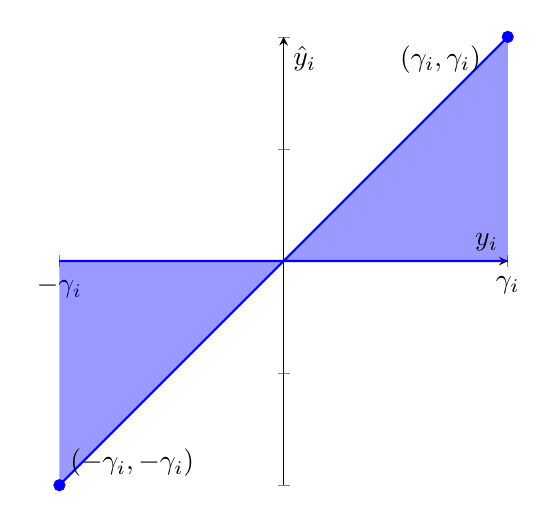
\begin{tikzpicture}
		\begin{axis}[
			xlabel={$y_i$},
			ylabel={$\hat{y}_i$},
			xmin=-2, xmax=2,
			ymin=-2, ymax=2,
			axis lines=center,
			samples=100, 
			unit vector ratio=1 1 1, scale=1, xtick   = {-2,2},
			xticklabels = {$-\gamma_i$,$\gamma_i$},
			yticklabels = {},
			]
			\addplot[blue, thick, fill=blue, fill opacity=0.4] {x} \closedcycle; 
			\addplot[blue, thick] {0}; 
			
			\addplot[only marks, mark=*, mark size=2pt, blue] coordinates {(-2,-2)};
			\node[label={above:$(-\gamma_i,-\gamma_i)$}] at (axis cs: -1.35, -2.1) {};
			
			\addplot[only marks, mark=*, mark size=2pt, blue] coordinates {(2,2)};
			\node[label={above:$(\gamma_i,\gamma_i)$}] at (axis cs: 1.4, 1.5) {};
		\end{axis}
	\end{tikzpicture}
	
	Now we can introduce this simplified model:
	
\begin{enumerate}
	\item For each input node, each output node, and each pre-activation and post-activation node in the hidden layers,  set one variable $y_i$. 
	\item Set constraints for input nodes.
	\item Set linear constraints . In this case, since the meaning of $y_i$ is $x_i-x'_i$, this constraints will not use the bias.
	\item Between pre- and post- activation nodes, set the MILP constraint described above.
\end{enumerate}
	
	The speed of this model is much faster, comparable to the MILP model for local robustness. However, in practice, this model sometimes lose much accuracy.
	
	\subsection{Another simplified model}

	The second simplified model is more complex than the first.
	
	We can use the following extra constraints (besides 4 constraints about $\hat{x}_i'=\ReLU(x_i')$) to build this relation:
	
	
	\begin{align*}
		&\hat{y}_i \geq -\hat{x}'_i \hspace*{1ex} \wedge \hspace*{1ex} \hat{y}_i \leq -\hat{x}'_i+a\beta_i  \hspace*{1ex}\wedge\hspace*{1ex} x_i'+y_i \leq a\beta_i \hspace*{1ex}\wedge\hspace*{1ex}  x_i'+y_i \geq (1-a)\alpha_i \\
		&\hat{y}_i \geq -\hat{x}'_i+(x_i'+y_i) \hspace*{1ex}\wedge\hspace*{1ex} \hat{y}_i \leq -\hat{x}'_i+(x_i'+y_i) +(a-1)\alpha_i \\
	\end{align*} 
	
	
	Moreover, we can add two more natural constraints: $x_i'+y_i \geq \alpha_i \hspace*{1ex}\wedge\hspace*{1ex}  x_i'+y_i \leq \beta_i.$
	
	
	
	A more direct way to establish the constraints is as follows: \begin{align*}
		& y_i+x'_i \leq a\beta_i \quad\wedge \quad y_i+x'_i\geq (1-a)\alpha_i\\	
		& x_i' \leq a'\beta_i \quad\wedge \quad x_i'\geq (1-a')\alpha_i\\
		&\hat{y}_i \leq a\gamma_i \quad\wedge \quad	\hat{y}_i \geq -a'\gamma_i \\
		&	\hat{y}_i \leq y_i+(1-a)\gamma_i \quad\wedge \quad	\hat{y}_i \geq y_i - (1-a')\gamma_i \\
		&	\hat{y}_i \leq -x'_i+a\beta_i \quad\wedge \quad	\hat{y}_i \geq -x'_i+(1-a')\alpha_i \\
		&	\hat{y}_i \leq y_i+x'_i+(1-a)(-\alpha_i)\quad\wedge \quad	\hat{y}_i \geq y_i+x'_i+a'(-\beta_i) \\
	\end{align*}The following two plots show its shape:
	
	\iffalse
	\hspace*{-10ex}
	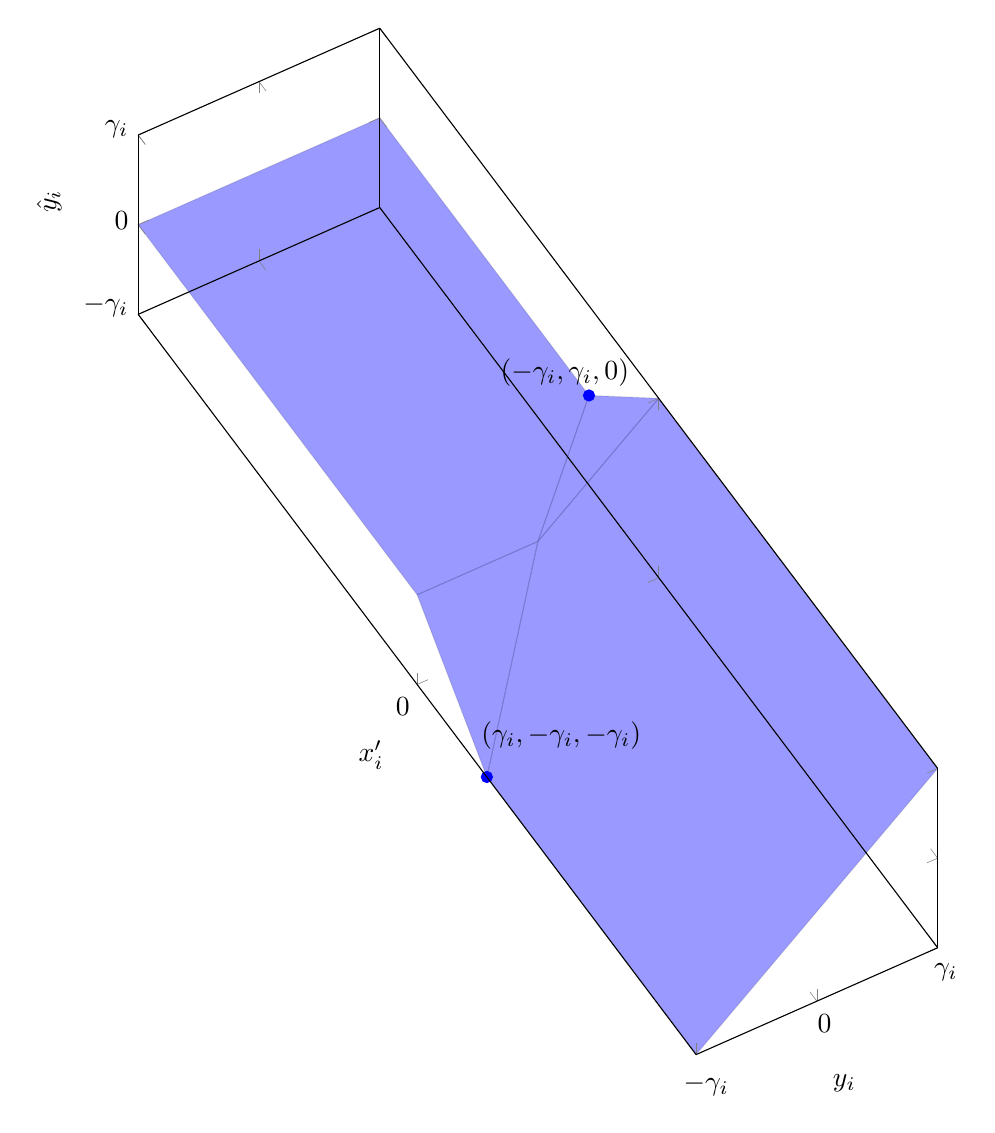
\begin{tikzpicture}
		\begin{axis}[	axis on top, xlabel = \(x'_i\),
			ylabel = {\(y_i\)}, zlabel = \(\hat{y}_i\),
			set layers=default,
			xmax = 4, xmin = -4,
			ymax = 1, ymin = -1,		
			zmax = 1, zmin = -1,
			unit vector ratio=1 1 1, scale=3,
			view={60}{50}, ytick   = {-1,0,1},
			yticklabels = {$-\gamma_i$,$0$,$\gamma_i$}, xtick = {0},
			xticklabels = {$0$}, ztick   = {-1,0,1},
			zticklabels = {$-\gamma_i$,$0$,$\gamma_i$},
			]
			\addplot3[fill=blue,opacity=0.1, fill opacity=0.4] 
			coordinates {
				(0,0,0) (-1,1,0) (-4,1,0) (-4,-1,0) (0,-1,0) (0,0,0)
			};
			
			\addplot3[fill=blue,opacity=0.1, fill opacity=0.4	] 
			coordinates { (0,0,0) (0,1,1) (4, 1, 1) (4, -1, -1) (1,-1,-1) (0,0,0)
			};
			
			\addplot3[fill=blue,opacity=0.1, fill opacity=0.4	] 
			coordinates { (0,0,0)  (-1,1,0) (0,1,1) (0,0,0)
			};
			
			\addplot3[fill=blue,opacity=0.1, fill opacity=0.4	] 
			coordinates { (0,0,0)  (0,-1,0) (1,-1,-1) (0,0,0)
			};
			
			\addplot3[only marks, mark=*, mark size=2pt, blue] coordinates {(1,-1,-1)};
			\node[label={$(\gamma_i,-\gamma_i, -\gamma_i)$}] at (axis cs: 1.2, -0.5 ,-1) {};
			
			\addplot3[only marks, mark=*, mark size=2pt, blue] coordinates {(-1,1,0)};
			\node[label={$(-\gamma_i,\gamma_i, 0)$}] at (axis cs: -1, 0.8 ,0) {};			
			
		\end{axis}
	\end{tikzpicture}
	\fi
	
	
	\hspace*{-15ex}
	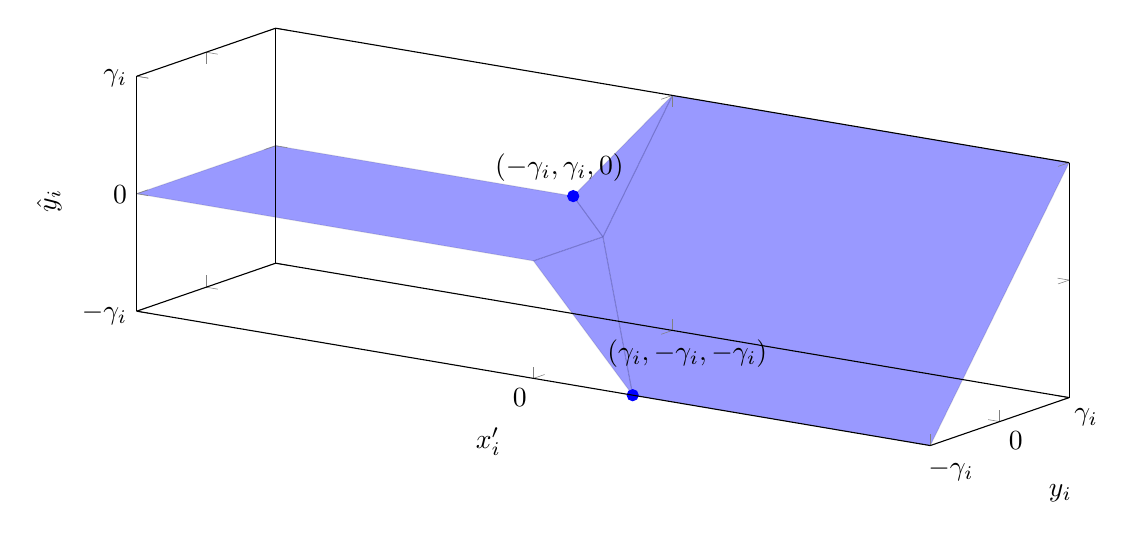
\begin{tikzpicture}
		\begin{axis}[	axis on top, xlabel = \(x'_i\),
			ylabel = {\(y_i\)}, zlabel = \(\hat{y}_i\),
			set layers=default,
			xmax = 4, xmin = -4,
			ymax = 1, ymin = -1,		
			zmax = 1, zmin = -1,
			unit vector ratio=1 1 1, scale=2.5,  ytick   = {-1,0,1},
			yticklabels = {$-\gamma_i$,$0$,$\gamma_i$}, xtick = {0},
			xticklabels = {$0$}, ztick   = {-1,0,1},
			zticklabels = {$-\gamma_i$,$0$,$\gamma_i$},
			view={35}{14},
			]
			\addplot3[ fill=blue,opacity=0.1, fill opacity=0.4] 
			coordinates {
				(0,0,0) (-1,1,0) (-4,1,0) (-4,-1,0) (0,-1,0) (0,0,0)
			};
			
			\addplot3[	fill=blue,opacity=0.1, fill opacity=0.4] 
			coordinates { (0,0,0) (0,1,1) (4, 1, 1) (4, -1, -1) (1,-1,-1) (0,0,0)
			};
			
			\addplot3[	fill=blue,opacity=0.1, fill opacity=0.4	] 
			coordinates { (0,0,0)  (-1,1,0) (0,1,1) (0,0,0)
			};
			
			\addplot3[	fill=blue,opacity=0.1, fill opacity=0.4	] 
			coordinates { (0,0,0)  (0,-1,0) (1,-1,-1) (0,0,0)
			};
			
			\addplot3[only marks, mark=*, mark size=2pt, blue] coordinates {(1,-1,-1)};
			\node[label={$(\gamma_i,-\gamma_i, -\gamma_i)$}] at (axis cs: 1.2, -0.5 ,-1) {};
			
			\addplot3[only marks, mark=*, mark size=2pt, blue] coordinates {(-1,1,0)};
			\node[label={$(-\gamma_i,\gamma_i, 0)$}] at (axis cs: -1, 0.8 ,0) {};			
			
		\end{axis}
	\end{tikzpicture}
	
	
	
	\section{Conclusion}
	
	TODO
	
	
	\bibliography{references}
	\bibliographystyle{plain}
	
	
	\bigskip
	
	\appendix
	
	
	
\end{document}


